
% this file is called up by thesis.tex
% content in this file will be fed into the main document

%: ----------------------- introduction file header -----------------------
\chapter{State of the Art}\label{ch:soa}

\graphicspath{{soa/figures/}}

% -------------------------------------------------------------
% -- Related Work
% -------------------------------------------------------------

In this chapter the main concepts that will be used throughout the rest of the thesis are introduced. 
We analyze the current state of the art and limitations in the area of exploration of large and multilingual document collections. First, the tasks derived from processing the texts and enabling a semantic-aware exploration of the corpus are described. Then, an overview of the existing methods that perform these tasks is introduced. And finally, for each research area involved, the limitations that must be addressed to achieve the ultimate goal of facilitating documentary exploration are presented. 

\section{Information Retrieval}

The analysis of human-readable documents is a well-known problem in Artificial Intelligence (AI) in general, and in the Information Retrieval (IR) and Natural Language Processing (NLP) fields in particular. As an academic field of study, information retrieval might be defined as finding documents of an unstructured nature, usually text, that satisfies an information need from within large collections \citep{manning2008}. As defined in this way, hundreds of millions of people engage in information retrieval every day when they use a web search engine or search their email. Information retrieval is fast becoming the dominant form of information access, surpassing traditional database searching where identifiers are needed to have results. 

There are some key concepts in this area.  The  records  that  IR  addresses  are  called \textit{documents}, and they are retrieved from an organized repository, most commonly called  \textit{collection} or \textit{corpus}. It is not restricted to static collections. The collection may be a stream of texts, e.g., scientific publications, patents, news dispatches, that are created periodically. DR focuses on retrieving documents from a collection based on their content. A request, typically called a \textit{query},  may specify desired characteristics of the documents to be retrieved, e.g., \textit{The documents should be about ‘Text Similarity’ and their author must be ‘Badenes’}. In this example, the query asks for documents whose content (the \textit{unstructured} part) is \textit{about} a certain topic and whose author (a \textit{structured} part) has a specified value. 

\textit{Unstructured Content} means that there is no well-defined syntax for a given document, let alone a syntax that all documents share. To the extent that documents share a syntax, there is no well-defined semantics associated with each syntactic component \citep{greengrass2000}. Now, think about how data is \textit{structured} in a database. All records of a given type have the same syntax, e.g., all rows in a table of a relational database will have the same columns \citep{Salton1983}.  Moreover,  each  component  of  a  record  will  have  a  definite meaning (i.e. semantics)  and  a  given  component  of  a  given  record  type  will  have  the  same semantics in every record of that type. The practical effect is that given the name of a component, a search engine can use the syntax to find the given component in a given record and retrieve its contents, its value. Similarly, given a component and a value, the search engine can find records such that the given component contains the given value. For example, a relational database can be asked to retrieve the contents of the \textit{year} column of a \textit{Thesis} table in an \textit{Academic} database. The search engine knows how to find the \textit{Thesis} table within  the  \textit{Academic}  database,  and  how  to  find  the  \textit{year}  column  within  each  record  of  the \textit{Thesis} table.  And  every  \textit{year}  column  within  the  \textit{Thesis}  table  will  have  the  same semantics, i.e., the year of publication of a thesis. 

But the column name \textit{year} may not be sufficient to identify the column. A \textit{Course} table in the same or a different database may also have a \textit{year} column. Hence in general, it may be necessary to specify a path, e.g., database name, table name,column name, to uniquely identify the syntactic component to the search engine. However, the syntax of a well-structured database is such that it is always possible to specify a given syntactic component uniquely and hence it is always possible for the search engine to find all occurrences of a given component. If the given component has a definite semantics, then it is always possible for the search engine to find data with that semantics, e.g., to find the years of all theses. 

By contrast, in a collection of unstructured natural language documents, there is no well-defined syntactic position where a search engine could find data with a given semantics, e.g., the years of theses. In a random collection of documents, there is no guarantee that they are all about the same topic, e.g., theses. Even if it is known that the documents are all about theses, there is no simple well-defined way of knowing where the year occurs in a given document, e.g., in what sentence or even in what paragraph. This is exactly what is meant by \textit{unstructured} texts.

An IR engine may use the query to classify the documents in a collection, returning to the user a subset of documents that satisfy some classification criterion. Documents that satisfy the query are said to be \textit{relevant}. The higher the proportion of documents returned to the user that judges as relevant, the better the classification criterion. Alternatively, the search engine may \textit{rank} the documents in a given collection. Document $D_1$ is higher ranking with respect to a given query $Q$ than document $D_2$, which means that $D_1$ is more likely to satisfy $Q$ than $D_2$. Or it may be interpreted as meaning that $D_1$ satisfies $Q$ more than $D_2$. Two measures of IR success, both based on the concept of relevance, are widely used: \textit{precision} and \textit{recall}. Precision is defined as the ratio of relevant items retrieved to all items retrieved, or the probability given that an item is retrieved that it will be relevant. Recall is defined as, the ratio of relevant items retrieved to all relevant items in a collection, or the probability given that an item is relevant that it will be retrieved \citep{saracevic1995}.

\section{Techniques for Document Retrieval}\label{sec:related-work}

There are two major categories of IR technology and research: semantic and statistical. Semantic approaches attempt to implement some degree of syntactic and semantic analysis. They try to reproduce to some degree the understanding of the natural language text that a human user would provide. In statistical approaches, the documents that are retrieved or that are highly ranked are those that match the query most closely in terms of some statistical measure. The work presented in this thesis follows this second approach. 

Statistical approaches break documents and queries into \textit{terms}. These terms are the population that is counted and measured statistically. Most commonly, the terms are words (or combination of adjacent words or characters) that occur in a given query or collection of documents and often require pre-processing. Words are reduced to a common base form by using a heuristic process that removes affixes, \textit{stemming}, or by returning its dictionary form, \textit{lemma} \citep{porter1997}. The objective is to eliminate the variation that arises from the occurrence of different grammatical  forms  of  the  same  word,  e.g.,  "program",  "programming",  "programs", and "programmed" should all be recognized as forms of the same word, "program". Another common form of pre-processing is the elimination of common words that have little power to discriminate relevant from non-relevant documents,e.g., "the", "a", "it". Hence, IR engines are usually provided with a \textit{stop-list} of such noise words. Note that both stemming/lemma and \textit{stopwords} are language-dependent. Once all terms have been pre-processed, numerical weights are assigned to each them. The same term may have a different weight in each distinct document in which it occurs. The weight is usually a measure of how effective the given term is likely to be in distinguishing the given document from other documents in the given collection, and is often normalized to be a fraction between zero and one. Statistical approaches fall into the following categories: \textbf{\textit{boolean}}, \textbf{\textit{vector space}} and \textbf{\textit{probabilistic}}.

An illustrative example\footnote{\url{https://github.com/cbadenes/phd-thesis/blob/master/notebooks/soa.ipynb}} may help to better understand these techniques. The publications listed in Section \ref{sec:publications} are used as a sample collection for applying information retrieval techniques. Documents are first pre-processed as described above to transform their texts into terms. Typically these terms are referred to as \textit{tokens}. Let's see the process by analyzing the following sentence taken from one of the documents: \textit{"Probabilistic Topic Models reduce that feature space by annotating documents with thematic information"}. Each word, identified using whitespace characters, is normalized using its dictionary form (stemming could also have been performed in this step). The sentence is then transformed into a list of lemmatized words: "\textit{['Probabilistic', 'Topic', 'Models', 'reduce', 'that', 'feature', 'space', 'by', 'annotate', 'document', 'with', 'thematic', 'information']}". Some words have changed and others have remained unchanged. For example, 'annotating' is reduced to 'annotate' and 'documents' to 'document'. However, 'Models' remains unchanged. The reason is that it is considered a proper noun since it starts with a capital letter. Once the words have been normalized, the words with less informative capacity are eliminated (e.g. \textit{'that'}, \textit{'by'} and \textit{'with'}). They usually belong to a stop-word list associated with a given language, but can also be domain-specific. The final list of terms are the tokens used to describe each of the documents.  Table \ref{table:ir-collection} shows the number of words and tokens of each document when preprocessed.


\begin{table}[!htbp]
\centering%
\begin{tabularx}{\linewidth}{lHll}
\toprule
\heading{Id} & \heading{Title} & \heading{Words} & \heading{Tokens} \\
\midrule
\midrule
$D_0$ & Cross-Evaluation of Term Extraction Tools by Measuring Terminological Saturation & 12,954 & 6,342 \\
\midrule
$D_1$ & Enhancing Public Procurement in the European Union through Constructing and Exploiting an Integrated Knowledge Graph & 5,827 & 3,406 \\
\midrule
$D_2$ & Drugs4Covid: Making drug information available from scientific publications & 5,417 & 3,260 \\
\midrule
$D_3$ & Distributing Text Mining tasks with librAIry & 2,448 & 1,477 \\
\midrule
$D_4$ & Large-Scale Semantic Exploration of Scientific Literature using Topic-based Hashing Algorithms & 9,041 & 5,604 \\
\midrule
$D_5$ & An initial Analysis of Topic-based Similarity among Scientific Documents based on their Rhetorical Discourse Parts & 2,641 & 1,425 \\
\midrule
$D_6$ & Efficient Clustering from Distributions over Topics & 5,346 & 2,986 \\
\midrule
$D_7$ & Legal Documents Retrieval Across Languages: Topic Hierarchies based on synsets & 1,445 & 787 \\
\midrule
$D_8$ & Scalable Cross-lingual Document Similarity through Language-specific Concept Hierarchies & 4,602 & 2,963 \\
\midrule
$D_9$ & Potentially inappropriate medications in older adults living with HIV & 3,087 & 2,018 \\
\midrule
$D_{10}$ & Semantic Saturation in Retrospective Text Document Collections & 7,700 & 1,753 \\
\midrule
\bottomrule
\end{tabularx}
\caption{Number of words and tokens of publications listed in Section \ref{sec:publications} when preprocessed.}
\label{table:ir-collection}
\end{table}


%Some sophisticated engines also extract \textit{phrases} as terms. A phrase is a combination of adjacent words which may be recognized by frequency of co-occurrence in a given collection or by presence in a phrase dictionary, e.g. "artificial intelligence". 
%At the other extreme, some engines break documents and queries into \textit{n-grams}, i.e., arbitrary strings of $n$ consecutive characters \citep{damashek1995}. A window of $n$ characters can be moved moved through the entire document, completely ignoring word, phrase, or punctuation boundaries, or can be constrained by word separators, or by other punctuation characters. In any case, since a single word or phrase can generate multiple n-grams, statistical clustering using n-grams has proved to be language-independent, and has even been used to sort documents by language, or by topic within language.

In a \textbf{boolean approach}, the query is formulated as a boolean combination of terms. Documents are reduced to true or false representations for each word depending on whether they contain it or not. A conventional boolean query uses the classical operators AND, OR, and NOT. The query "$t_1$ AND $t_2$" is satisfied by a given document $D_1$ if and only if $D_1$ contains both terms $t_1$ and $t_2$. Similarly, the query "$t_1$ OR $t_2$" is satisfied by $D_1$ if and only if it contains $t_1$ or $t_2$ or both. The query "$t_1$ AND NOT $t_2$" satisfies $D_1$ if and only if it contains $t_1$ and does not contain $t_2$. In the above example, the query needed to find the articles dealing with topic hierarchies or multilingualism would be: "\textit{multilingual OR (topic AND hierarchy)}" (note the normalization of terms). More complex boolean queries can be built up out of these operators and evaluated according to the classical rules of boolean algebra. Such a boolean query is either true or false. Correspondingly, a document either satisfies such a query, i.e. is \textit{relevant}, or does not satisfy it, i.e. is \textit{non-relevant}. For the above query, documents $D_1$, $D_4$, $D_6$, $D_7$ and $D_8$ are found relevant. However \textbf{no ranking is possible using this representation}, which is a significant limitation for this approach \citep{harmon1995}. 

\textbf{Vector space models (VSM)} \citep{Salton1983} were proposed to represent texts as vectors where each entry corresponds to a different term and the number at that entry corresponds to how many times that term is present in the text. The objective was twofold: on the one hand, making document collections manageable since we move from having lots of terms for each text to only one vector per document with a defined dimension; on the other hand, having representations based on metric spaces where calculations can be made, for example comparisons by measuring vector distances. The definition and number of dimensions for each vector are key aspects in a VSM. Based on the use of this type of model, traditional document retrieval tasks over collections of textual documents highly rely on individual features like term frequencies (TF) \citep{Hearst1999}. A representational space is created where each term in the vocabulary is projected by a separate and orthogonal dimension. The relevance of the documents according to a given query can be calculated by adding the frequencies of the query terms for each document. Thus, the search for articles dealing with topic hierarchies or multilingualism return the sorted list of relevant documents: (1)$D_4$, (2)$D_8$, (3)$D_6$, (4)$D_7$ and (5)$D_1$. But in this approach \textbf{all terms in a document are treated as equally descriptive}. To overcome this limitation, Term-Frequency Inverse-Document Frequency (TF-IDF) \citep{lee1995} relativizes the relevance of each term with respect to the entire corpus. TF-IDF calculates the importance of a term for a document, based on the number of times the term appears in the document itself (term frequency - TF) and the number of documents in the corpus, which contain the term (document frequency - DF). The above query, taking into account this representation, slightly varies the order of relevance of the documents: (1)$D_8$, (2)$D_7$, (3)$D_4$, (4)$D_6$ and (5)$D_1$. $D_8$ and $D_7$ are now the most relevant documents because, although the query terms are are less frequent than in $D_4$, their relative frequency (considering the length of the articles) is higher. However the \textbf{absence of semantic information and the high-number of dimensions are the main drawbacks} of these approaches that lead to the emergence of other techniques. In the above example, with a collection of only 11 documents, the dimension of the vectors is equal to 6,182 (i.e. the number of unique tokens in the whole corpus).

New ways of characterizing documents appeared more recently based on the automatic generation of models discovering the main themes covered in the corpus. Among them, text embedding proposes transforming texts into low-dimensional vectors by prediction methods based on (i) word sequences or (ii) bag-of-words. The first approach assumes words with similar meanings tend to occur in similar contexts. It considers that word order is relevant, and is based on Neural Models (NM) that learn word vectors from pairs of target and context words. Context words are taken as words observed to surround a target word. Document vectors are usually created by taking the word vectors they contain or by considering them as target and context items. Skip-gram with negative sampling (Word2Vec) \citep{Mikolov2013c} and Global Vectors (GloVe) \citep{pennington2014} are indeed the most popular methods to learn word embeddings due to its training efficiency and robustness \citep{levy2015}. Figure \ref{fig:doc2vec} shows the two-dimensional projection of the example articles described by word embeddings. In particular, document representations are calculated via distributed memory using the Paragraph Vector \citep{LeMikolov2014} algorithm. The original dimensions of the vector space were reduced by Principal Component Analysis (PCA) to the dimensions of the graph. This representation brings together documents that share not only the same vocabulary, but also the way of using it, since it takes into account sequences of words, and separates documents that use different relevant terms or in different ways. For this reason, document $D_0$ appears clearly distanced from the rest, since it is more focused on saturation measures from term collections. And the same happens with document $D_7$, which presents a specific case in the legal domain.



\begin{figure}[!htbp]
\centering
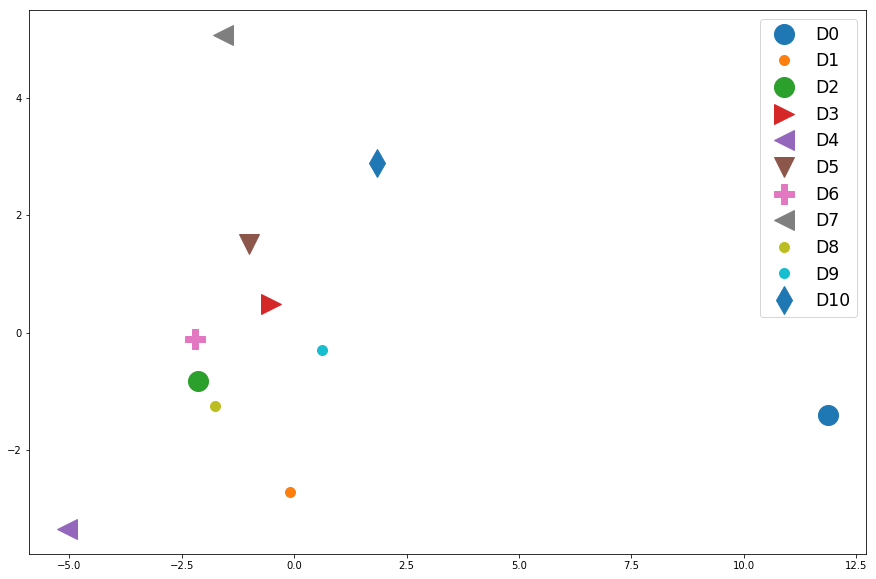
\includegraphics[scale=0.34]{doc2vec.png}
\caption{Documents listed in Section \ref{sec:publications} described by word embeddings and projected in a two-dimensional space by PCA. }
\label{fig:doc2vec}
\end{figure}


The second approach does not consider the order of the words to be relevant, but their frequency. It assumes words with similar meanings will occur in similar documents, and avoids considering the same terms or the same word sequences to relate documents. Topic models \citep{Deerwester1990} are the main methods that are based on this approach. \textbf{Probabilistic Topic Models (PTM)} \citep{Hofmann2001,Blei2003} are statistical methods based on bag-of-words that analyze the words of the original texts to discover the themes that run through them, how those themes are connected to each other, or how they change over time. PTM do not require any prior annotations or labeling of the documents. The topics emerge, as hidden structures, from the analysis of the original texts. These structures are topic distributions, per-document topic distributions or per-document per-word topic assignments. In turn, a topic is a distribution over terms that is biased around those words associated to a single theme. To better understand what topic means in this context, table \ref{table:sample-topics} shows the topics that have emerged when creating a topic model with the collection of example publications. Each topic is described by its five most representative words, i.e., those words most present in the documents that mainly contain each topic.

\begin{table}[!htbp]
\centering%
\begin{tabularx}{\linewidth}{HHHHH}
\toprule
\heading{Topic 0} & \heading{Topic 1} & \heading{Topic 2} & \heading{Topic 3} & \heading{Topic 4} \\
\midrule
\midrule
topic (27) & drug (15) & term (21) & synset (9) & document (1)\\
\midrule
document (20) & disease (9) & collection (11) & topic (8) & topic (1) \\
\midrule
base (17) & old (6) & document (10)  & document (8) & term (1)\\
\midrule
distribution (8) & PLWH (5) & value (9) & lingual (7) & base (1) \\
\midrule
model (8) & medication (5) & saturation (9) & category (6) & collection (1)\\
\midrule
\bottomrule
\end{tabularx}
\caption{Probabilistic topics created from the collection of articles listed in Section \ref{sec:publications}. For each topic the five most representative words are shown together with their normalized relevance (0-1000).}
\label{table:sample-topics}
\end{table}


This interpretable hidden structure annotates each document in the collection and these annotations can be used to perform deeper analysis about relationships between documents. Topic-based representations bring a lot of potential when applied over different IR tasks, as evidenced by recent works in different domains such as scholarly  \citep{Gatti2015}, health \citep{Lu2016, TapiNzali2017}, legal \citep{ONeill2017, Greene2016}, news \citep{He2017} and social networks \citep{Cheng2014a}. Moreover, some hybrid proposals have been recently used to model topics from word embeddings\citep{Dieng2020TopicMI}. Following the previous example, Figure \ref{doctopics} shows the articles projected in a two-dimensional space from their probabilistic topic-based representations. Unlike the distribution shown in Figure \ref{fig:doc2vec}, several documents now appear at the same position (e.g. $D_2-D_9$ and $D_3-D_4-D_6-D_8$). Being such a small collection of documents, 11 items, there are topics that are strongly present in the documents to differentiate them from the others. Thus, \textit{topic 1} groups documents $D_2$ and $D_9$ since it is related to the health domain. The same happens with documents $D_3$, $D_4$, $D_6$ and $D_8$ clearly focused on the efficient clustering of documents by probabilistic topics. In this case, \textit{topic 0} brings these documents together. The rest of the papers have a more balanced distribution of topics, indicating that they are less specific in a given domain.

\begin{figure}[!htbp]
\centering
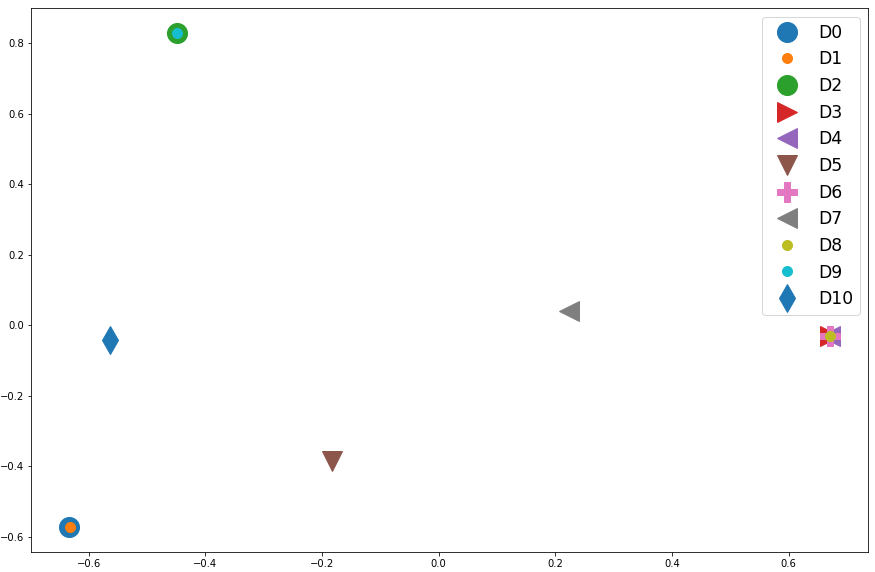
\includegraphics[scale=0.34]{doctopics.png}
\caption{Documents listed in Section \ref{sec:publications} described by probabilistic topics (Table \ref{table:sample-topics}) and projected in a two-dimensional space by PCA. }
\label{fig:doctopics}
\end{figure}

As just shown, the bag-of-words approach avoids the restriction of word sequences to relate documents. Documents that do not necessarily use the same words or in the same way can be strongly related if they mainly use the words that are more relevant for the same topic. The connection between documents is now the topic, not the word. Topic modeling provides an algorithmic solution to organize and annotate large collections of textual documents according to their topics. Our work is based on this approach since \textit{we are not only interested in representing words and documents, but we also seek structures that allows considering knowledge about the collection}.



\section{Techniques for Probabilistic Topic Models}\label{sec:techniques-prob-topics}

The simplest generative topic model proposed in the state of the art is \textit{Latent Dirichlet Allocation} (LDA) \citep{Blei2003}. Along with \textit{Latent Semantic Analysis} (LSA) \citep{Deerwester1990} and \textit{Probabilistic Latent Semantic Analysis} (pLSA) \citep{Hofmann2001} are part of the field known as topic modeling. They are well-known latent variable models for high dimensional data, such as the bag-of-words representation for textual data or any other count-based data representation. They try to capture the intuition that documents can exhibit multiple themes. Each document exhibits each topic in different proportion, and each word in each document is drawn from one of the topics, where the selected topic is chosen from the per-document distribution over topics. All the documents in a collection share the same set of topics, but each document exhibits these topics in a different proportion. Texts are described as a vector of counts with $W$ components, where $W$ is the number of words in the vocabulary. Each document in the corpus is modeled as a mixture over $K$ topics, and each topic $k$ is a distribution over the vocabulary of $W$ words. Formally, a topic is a multinomial distribution over words of a fixed vocabulary representing some concept. Depending on the function used to describe that distribution there are different algorithms to create topic models. LSA and pLSA propose a singular value decomposition. However, they have over-fitting issues. LDA was later proposed to overcome these issues. Influenced by the generative Bayesian framework it  suggests the use of a Dirichlet function as a continuous multivariate probability distribution parameterized by a vector of positive reals whose elements sum to 1.  It is continuous because the relative likelihood for a random variable to take on a given value is described by a probability density function, and is multivariate because it has a list of variables with unknown values. In fact, the Dirichlet distribution is the conjugate prior of the categorical distribution and multinomial distribution and allows LDA to infer topic distributions in texts that have not been used during training, unlike LSA and pLSA.

Topic models are not restrictive clustering models where each document is assigned to one cluster, but allow documents to exhibit multiple topics. The topics covered in a set of documents are discovered from the own corpus and feature vectors are topic distributions expressed as vector of probabilities.


\subsection{Document Similarity Calculation based on LDA}\label{sec:doc-sim-lda}

Since documents are described by topic distributions, the semantic similarity between two texts is based on the distance of their vector representations of the topics, which can be also seen as two probability mass functions. A commonly used metric is the \textit{Kullback-Liebler} (KL) divergence:

\begin{equation}
KL(P,Q) = \sum\limits_{i=1}^K p(x_{i}) \log \frac{p(x_{i})}{q(x_{i})}
\label{eq:kl}
\end{equation}
where  $K$ is the number of topics and $p,q$ are the topics distributions.

However, it presents two major problems: (1) when a topic distribution is zero, KL divergence is not defined and (2) it is not symmetric, which does not fit well with semantic similarity measures that are usually symmetric \citep{Rus2013}.

\textit{Jensen-Shannon} (JS) divergence \citep{Rao1982,Lin1991} solves these problems considering the average of the distributions as below \citep{Celikyilmaz2010}:

\begin{equation}
JS(P,Q) = \sum\limits_{i=1}^K p_{i}*\log \frac{2*p_{i}}{p_{i}+q_{i}}  +  \sum\limits_{i=1}^K q_{i}*\log \frac{2*q_{i}}{q_{i}+p_{i}}
\label{eq:jsdivergence}
\end{equation}


It can be transformed into a similarity measure as follows \citep{Dagan1998} :

\begin{equation}
sim_{JS}(D_i , D_j) = 10^{- JS(p,q)}
\label{eq:simjs}
\end{equation}
where  $D_i,D_j$ are the documents and $p,q$ the topic distributions of each of them.


\textit{Hellinger} (He) distance is also symmetric and is used along with JS divergence in various fields where a comparison between two probability distributions is required \citep{Blei2007a,Hall2008,Boyd-Graber2010}:

\begin{equation}
	He(P, Q) = \frac{1}{\sqrt{2}}\cdot\sqrt{\sum\limits_{i=1}^K (\sqrt{p_i} - \sqrt{q_i})^2)}
	\label{eq:hedistance}
\end{equation}

It can be transformed into a similarity measure by subtracting it from 1 \citep{Rus2013} such that a zero distance means max. similarity score and vice versa:

\begin{equation}
	sim_{He}(D_i, D_j) = 1 - He(p,q)
	\label{eq:simhe}
\end{equation}

However, all these metrics are not well-defined distance metrics, that is, they do not satisfy triangle inequality \citep{Charikar2002}. This inequality considers $d(x, z) <= d(x, y) + d(y, z)$ for a metric $d$ \citep{Griffiths2007} and places strong constraints on distance measures and on the locations of points in a space given a set of distances. As a metric axiom, the triangle inequality must be satisfied in order to take advantage of the inferences that can be deduced from it. Thus, if similarity is assumed to be a monotonically decreasing function of distance, this inequality avoids the calculation of all pairs of similarities by considering that if $x$ is similar to $y$ and $y$ is similar to $z$, then $x$ must be similar to $z$. 

\text{S2JSD} was introduced by \citep{Endres2003} to satisfy the triangle inequality. It is the square root of two times the $JS$ divergence:

%S2JSD formula
\begin{equation}
    S2JSD(P,Q) = \sqrt{2*JS(P,Q)}
\label{eq:s2jsd}
\end{equation}

\section{Research Areas}
\label{sec:research-topic}

This thesis aims to enable a semantic-aware exploration of the knowledge arising from large and multilingual document collections by exploiting the capabilities of topic models and their metric spaces. There are several research areas of ongoing related work. 

The first one is \textbf{topic creation and reuse}, key for understanding the steps needed to transform the unstructured data from a text into numerical values based on probabilistic topics. \textit{The way in which topic models are created and reused is crucial to addressing large-scale analysis}. 

The second area is \textbf{topic explainability}, which refers to the capacity of topics to capture and describe the content of a text. Topic explainability is important for \textit{making understandable the relationships that are derived from the inference of topic distributions}. 

The third area is \textbf{document similarity}, where the ability to measure the \textit{semantic difference between texts from the distance between their topic distributions is addressed}. 

Finally, the fourth area is \textbf{multilingual topics}, as we aim to explore collections of texts written in different languages through their topic-based relationships. A \textit{strategy to relate the topics of each language is tackled}. 

These four areas are closely related to each other. Having efficient thematic representations of texts, distance metrics based on shared themes, and mechanisms to abstract the particularities of a language to represent the themes, may help to organize large multilingual document collections.

Each area and its limitations are described below. A summary can be found in Table~\ref{table:limitations}.

\begin{table}[!htbp]
\centering%
\begin{tabularx}{\linewidth}{bbb}
\toprule
\heading{Area} & \heading{Scope}& \heading{Limitation} \\
\midrule
\midrule
topic creation & process texts and train topic models from large corpora & horizontal scalability (i.e. distributed computing) generally ignored in favor of vertical scalability (i.e. more computational power)  \\
\midrule
topic reuse & calculate topic distributions using existing topic models & no unified or standardized models for exchanging topic models \\
\midrule
topic explainability & describe and relate documents by topics & high dimensional models makes them difficult to interpret\\
\midrule
document similarity & compare topic distributions by measuring their distances & unaffordable complexity in huge collections  \\
\midrule
multilingual topics & topic distributions across languages & parallel or comparable training data required\\
\bottomrule
\end{tabularx}
\caption{Research areas and limitations.}
\label{table:limitations}
\end{table}



\subsection{Topic Creation and Reuse}
\label{sec:topic-reuse}

Textual content usually includes non-relevant information. Keeping only what can bring value for the involved agents (general consumers, experts, companies, investors...) becomes a challenge. A necessary first step before leveraging documents for knowledge-intensive tasks is to preprocess them following different techniques. Recent studies \citep{Westergaard2017} have shown that mining full-text articles gives consistently better results than only using sections or summaries. Given the size limitations and concise nature of summaries, they often omit descriptions or results that are considered to be less relevant but still are important for some IR tasks \citep{Divoli2012}.  Since this behavior is present in multiple domains, \textit{our interest is focused on processing full texts, not only summaries or parts of texts}, as we will show in the remainder of this thesis.

There is a broad set of algorithms able to analyze text for producing annotations at very different levels of granularity: from minimal units such as terms and entities, to descriptors at the level of the entire collection, such as summaries or topics. This includes methods and tools to perform Part-of-Speech (PoS) tagging, to recognize Named Entities (NER), or to create topic models following LDA or any other approach (e.g. LSA or pLSA). But their implementations have been designed to work in an isolated, non-collaborative way \citep{Manning2014TheToolkit, Agerri2014}. They have not paid special attention to facilitating their interoperability and they use closed data formats that increase the technological dependence and limits the reuse possibilities. For example, a topic model created by Mallet\footnote{\url{http://mallet.cs.umass.edu}} can only make inferences if it is used from Mallet itself or using its libraries, since \textbf{\textit{there is no unified or standardized format for distributing topic models}}. In that example, the fact that Mallet is implemented in Java prevents reusing their models from Python or any other programming language.

Some very recent approaches offer the creation and exploitation of topic models through an API based on libraries\footnote{\url{https://bab2min.github.io/tomotopy}} or web services\footnote{\url{https://github.com/D2KLab/ToModAPI}}\citep{Lisena:NLPOSS2020}. However they are focused on the operations that can be performed on the model rather than abstracting the topic model as a resource. Others provide local\footnote{\url{https://onnx.ai/}} or remote\footnote{\url{https://vespa.ai}} ecosystems to create and reuse learning models, but their data format is not open and cannot be (re)used out of the environment. To the best of our knowledge, the efforts made do not propose an unified model to exchange topic models, understood as an already accepted standards-based format. In this thesis we propose \textit{reusable topic models and a scalable framework to create and use them}.  
 

\subsection{Topic Explainability}
\label{sec:topic-explainability}

Even though the distance metrics mentioned in Section~\ref{sec:related-work} have been proposed and used in the SoA, making sense out of the similarity score based on compare topic distributions is not easy. As shown in figures \ref{fig:topic_distances} and \ref{fig:topic_distances2}, given a set of pairs of documents, their similarity scores vary according to the number of topics. So the distances between the same pairs fluctuate from being more to less distant when changing the number of topics, and are hence difficult to use to relate documents semantically. Understanding which of those distances is better for representing the underlying collection is a challenge.


\begin{figure}[]
\begin{subfigure}[b]{1.0\linewidth}
\centering
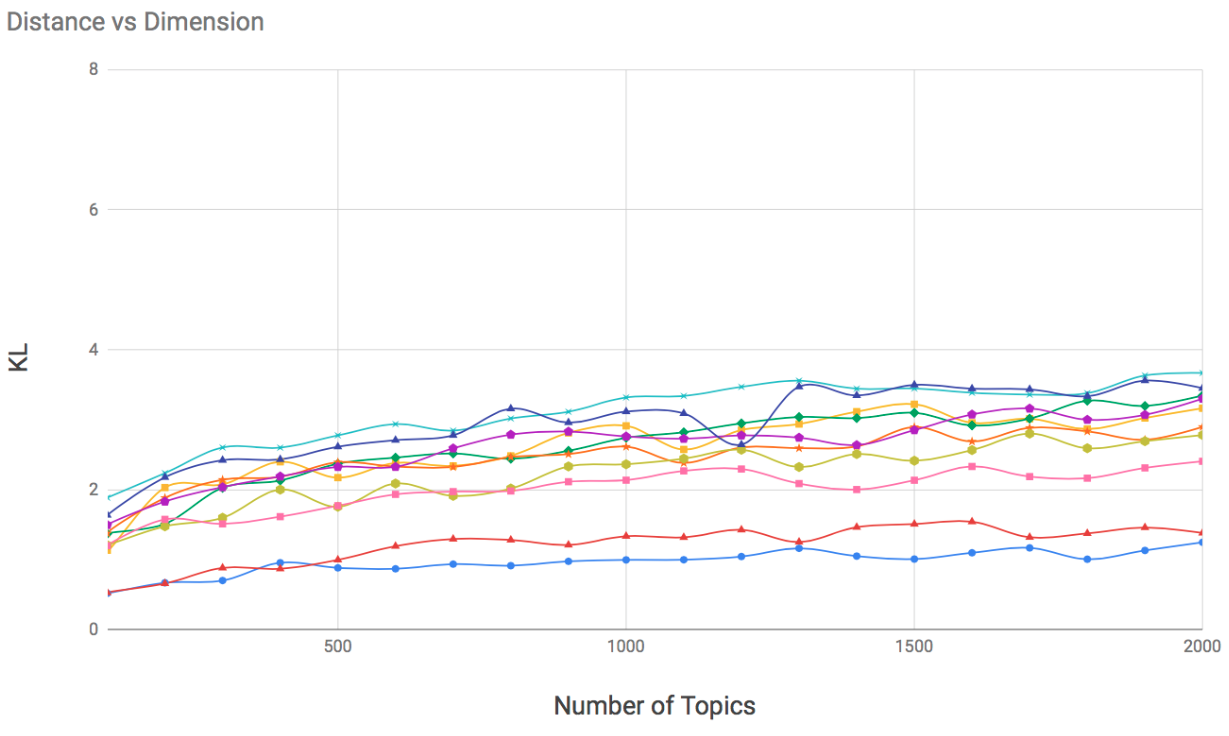
\includegraphics[width=\linewidth]{KL_100_2k.png}
\caption{Kullback-Liebler divergence}
\vspace{4ex}
\end{subfigure}
\begin{subfigure}[b]{1.0\linewidth}
\centering
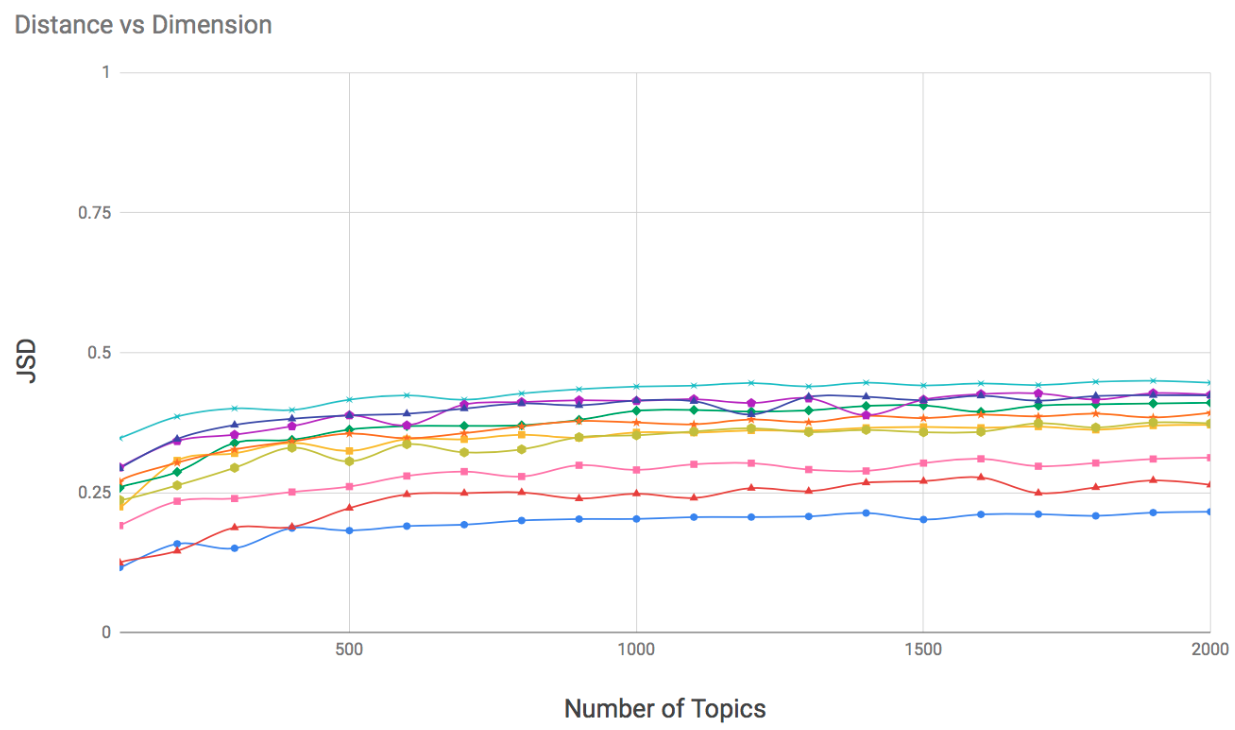
\includegraphics[width=\linewidth]{JSD_100_2k.png}
\caption{Jensen-Shannon divergence}
\vspace{4ex}
\end{subfigure}
\caption{Evolution of the distances based on KL (a) and JS (b) metrics between a set of document pairs when increasing the number of topics in the models  \citep{Badenes-Olmedo2020}.}
\label{fig:topic_distances}
\end{figure}

\begin{figure}[]
\begin{subfigure}[b]{1.0\linewidth}
\centering
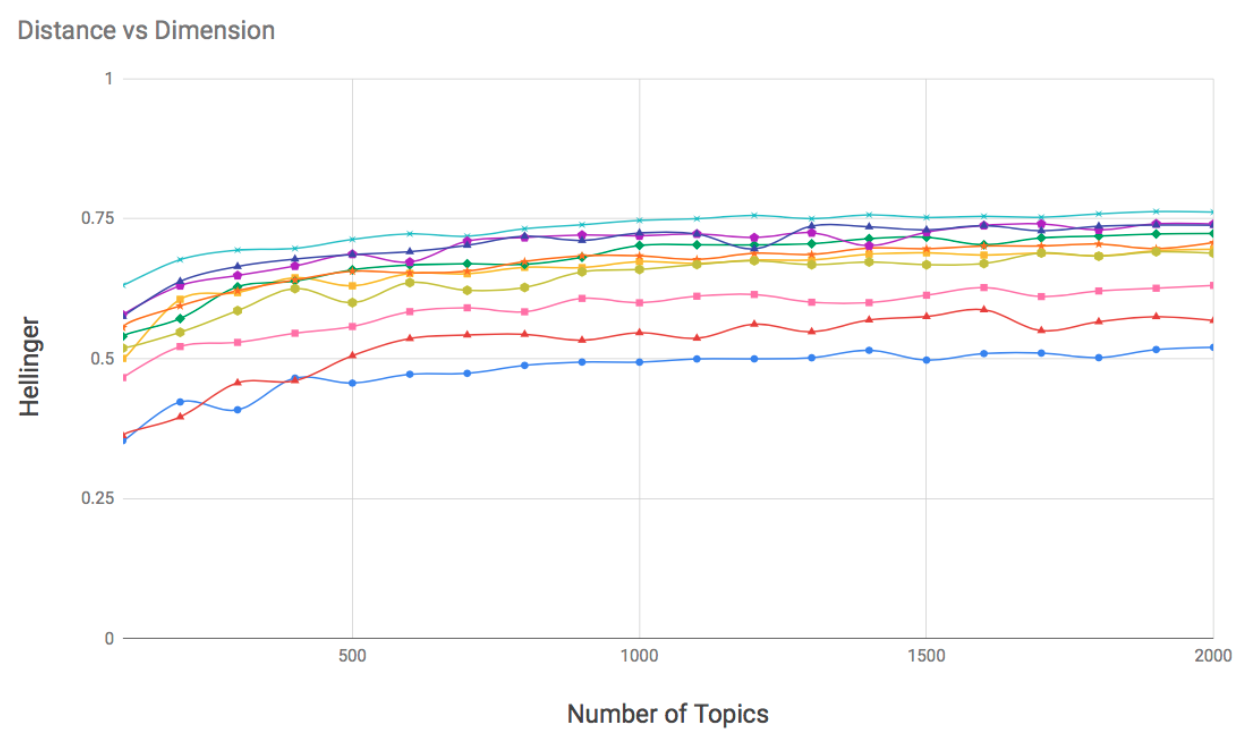
\includegraphics[width=\linewidth]{He_100_2k.png}
\caption{Hellinger distance}
\vspace{4ex}
\end{subfigure}
\begin{subfigure}[b]{1.0\linewidth}
\centering
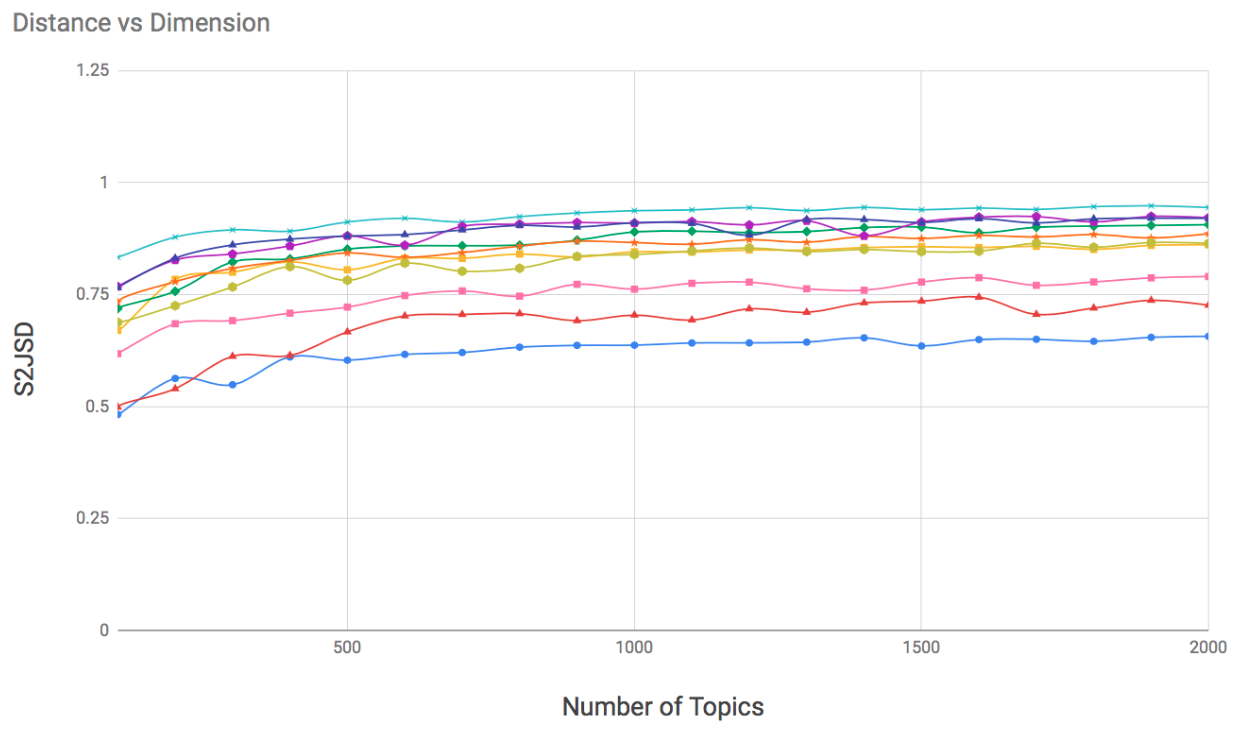
\includegraphics[width=\linewidth]{S2JSD_100_2k.png}
\caption{S2JSD distance}
\vspace{4ex}
\end{subfigure}
\caption{Evolution of the distances based on He (a) and S2JSD (b) metrics between a set of document pairs when increasing the number of topics in the models  \citep{Badenes-Olmedo2020}.}
\label{fig:topic_distances2}
\end{figure}


Distances between documents based on topic distributions generally increase as the number of dimensions of the space increases because it is a vector space. This is due to the fact that as the number of topics describing the model increases, the more specific the topics will be. Topics shared by a pair of documents can be broken down into more specific topics that are not shared by those documents. \textit{Document similarity is then dependent on the model used to represent documents when considering this type of metrics}. 

Each topic is drawn from a Dirichlet distribution with parameter $\beta$, while each document's mixture is sampled from a Dirichlet distribution with parameter $\alpha$. These two priors, $\alpha$ and $\beta$, are also known as hyper-parameters of a topic model and they set the probability that a document or a word, respectively, contains more than one topic. We know that absolute distances between documents vary when we tune those hyper-parameters differently, but we also see that ``relative distances" also change. Imagine that we have three documents, A, B and C, described by a topic model, M1. The distance from the topic distribution of A to B is less than from A to C. However, in a second topic model, M2, trained with the same documents than M1 but with different hyper-parameters, the distance from the topic distribution of A to C is less than to B (cross-lines in figures \ref{fig:topic_distances} and \ref{fig:topic_distances2}). This behaviour highlights the \textbf{\textit{difficulty of establishing absolute similarity thresholds and the complexity to measure distances taking into account all dimensions of a topic model}}. If we consider that documents are similar when their distance is lower than 0.2,for example, a pair of documents may be similar when they are represented in low-dimensional topic models, and not similar when high-dimensional models are used to represent them. Distance thresholds should be model-dependent rather than general, and metrics flexible enough to handle dimensional changes. In this thesis we go beyond the thematic and low-dimensional feature space created by topic models and propose a \textit{hierarchical feature space suitable for big real-world data sets, where documents are only described by their most relevant topics}.


\subsection{Document Similarity}
\label{sec:document-similarity}

In addition, document similarity comparisons are too costly to be performed in huge collections of data and require more efficient approaches than having to calculate all pairwise similarities. Using a naive approach creating a similarity matrix with all document comparisons takes $O(n^2)$ time (where $n$ is the number of documents), so obtaining all possible pairs of similarities in a large collection of documents (e.g. a corpus of 32 million patents) can be unfeasible because of the quadratic cost of comparing every pair of elements. Many different approaches have been proposed to reduce this complexity. For instance, computation can be approximated by a nearest neighbors (ANN) search problem \citep{Indyk1998}. ANN search is an optimization problem that finds nearest neighbors of a given query in a metric space of $n$ points. 

Due to the low storage cost and fast retrieval speed, hashing is one of the most popular solutions for ANN search \citep{Zhen2016}. This technique transforms data points from the original feature space into a binary-code space, so that similar data points have larger probability of collision (i.e. having the same hash code). This type of formulation for the document similarity comparison problem has proven to yield good results in the metric space \citep{Krstovski2011} due to the fact that ANN search has been designed to handle distance metrics (e.g. cosine, Euclidean, Manhattan). But distance metrics between topic distributions should be information-theoretically motivated metrics (e.g. Hellinger, Kullback-Leibler divergence, Jensen-Shannon divergence) since they compare density functions. 

These challenges can be tackled by hashing methods based on clusters of topics to measure similarity, instead of directly using their weights. Hashing methods transform the data points from the original feature space into a binary-code Hamming space, where the similarities in the original space are preserved. They can learn hash functions (data-dependent) or use projections (data-independent) from the training data \citep{Wang2016}. Data-independent methods, unlike data-dependent ones do not need to be re-calculated when data changes, i.e. adding or removing documents to the collection. Taking large-scale scenarios into account (e.g. Document clustering, Content-based Recommendation, Duplicate Detection), data independency is a key feature along with the ability to infer hash codes individually (for each document) rather than on a set of documents. Data-independent hashing methods depend on two key elements: (1) data type and (2) distance metric. For vector-type data, as introduced in section \ref{sec:related-work}, based on $l_p$ distance with $p \epsilon [0,2)$ lots of hashing methods have been proposed, such as p-stable Locality-Sensitive Hashing (LSH) \citep{Datar2004}, Leech lattice LSH \citep{Andoni2006}, Spherical LSH \citep{Terasawa2007}, and Beyond LSH \citep{Andoni2014}. Based on the $\theta$ distance many methods have been developed such as Kernel LSH \citep{Kulis2012} and Hyperplane hashing \citep{Vijayanarasimhan2014}. But only few methods handle density metrics in a simplex space, where topic distributions are projected. A first approach transformed the $He$ divergence into an Euclidean distance so that existing ANN techniques, such as LSH and k-d tree, could be applied \citep{Krstovski2013a}. But this solution does not consider the special attributions of probability distributions, such as Non-negative and Sum-equal-one. Recently, a hashing schema \citep{Mao2017} has been proposed taking into account the symmetry, non-negativity and triangle inequality features of the S2JSD metric for probability distributions. For set-type data, Jaccard Coefficient is the main metric used. Some examples are K-min Sketch \citep{Li2012}, Min-max hash \citep{Ji2013}, B-bit minwise hashing \citep{Li2010b} and Sim-min-hash \citep{Zhao2013}.

All of them have demonstrated efficiency in the search for similar documents, but none of them considers the search for documents (1) by thematic areas or (2) by similarity levels, nor they offer (3) an \textbf{\textit{explanation about the similarity obtained beyond the vectors used to calculate it}}. In addition, binary-hash codes drop a very precious information: the topic relevance. This thesis proposes a \textit{hash function-based approach that allows efficiently searching for related documents while maintaining topic-based annotation, preserving the notion of why two documents are related}.


\subsection{Multilingual Topic Alignment}
\label{sec:multi-topic-alignment}

When the IR task is also cross-language, document retrieval must be independent of the language of the user's query. At execution time, the query in the source language is typically translated into a target language with the help of a dictionary or a machine-translation system. But for many languages we may not have access to translation dictionaries or a full translation system, or they can be expensive to execute, or expensive to train (lot of data required) in an online search system. In such situations it is useful to rely on smaller annotation units derived from the text so the full content does not need to be translated, for instance by finding correspondences with regard to the topics that are present in both the query and the documents being searched.

Some methods use document-aligned corpora, where documents are grouped and constrained to the same topic distribution during training to align the different languages \citep{mimno-etal-2009-polylingual, Ni2009, Fukumasu2012, Zhang2013}, or theme-aligned corpora, where similar themes and ideas appear in all languages \citep{Graber2009}. Multilingual Probabilistic Topic Models (MuPTM) \citep{Vulic2015} emerged in this area as a group of language-independent generative machine learning models that can be used on theme-aligned multilingual texts. They are based on LDA, adding supervised associations between languages by using \textit{parallel} corpora, with sentence-aligned documents (e.g. Europarl\footnote{https://ec.europa.eu/jrc/en/language-technologies/dcep} corpus), or \textit{comparable} corpora, with theme-aligned documents (e.g. Wikipedia\footnote{https://www.wikipedia.org/} articles), in multiple languages. Once a MuPTM has been generated, documents can be represented by data points in a single feature space based on topics to detect similarities among them exploiting inference results and using distance metrics. Due to its generic language-independent nature and the power of inference on unseen documents, MuPTM's have found many interesting applications in many different cross-lingual tasks. They have been used on cross-lingual event clustering \citep{Smet2009}, document classification \citep{10.1007/978-3-642-20841-6_45, Ni:2011:CLT:1935826.1935887},  semantic similarity of words \citep{mimno-etal-2009-polylingual, Vulic:2012:DHC:2380816.2380872}, information retrieval \citep{10.1007/978-3-642-36973-5_9, ganguly-etal-2012-cross}, document matching \citep{Platt:2010:TDR:1870658.1870683, zhu-etal-2013-building}, and others. 

There are also methods based on word alignments from bilingual dictionaries instead of aligned corpora. Topic models emerge as distributions over crosslingual equivalence classes of words \citep{Jagarlamudi2010, zhang-etal-2010-cross, shi-etal-2016-detecting, hao-paul-2018-learning}. Others propose to translate only the words used to characterize the topics across the languages, such as anchor words \citep{NEURIPS2018_28b9f8aa} or top words \citep{yang2019multilingual}. A recent approach is placed between word and document alignments since it proposes crosslingual topic models using the language-independent categories assigned to each Wikipedia article \citep{2020arXiv200911207P}. Instead of using bags-of-words to represent texts, which would be language dependent, it explores the references of each article and represents them through bags-of-links, using the categories of each reference to represent the texts.

However, \textbf{\textit{the requirement of parallel/comparable corpora or dictionaries limits the usage of these models in many cross-lingual situations}}. There are not many document collections that can be used for training since large parallel corpora are rare in most of the use cases, especially for languages with fewer resources. Moreover, in order to incorporate new languages or update the existing associations, these models must be (re)trained with documents from all languages at the same time, making it difficult to scale to large corpora \citep{Hao2018, Moritz2017}. Inspired by the work of \citep{Boyd-Graber2010}, where the use of concepts to align topics from different languages is proposed, we take MuPTM a step further by making it cross-lingual through representations based on topic hierarchies. We do not only use conceptual representations of the top words in a topic, but we group the words hierarchically by relevance and compare their conceptual representations at those levels. Documents are represented by topics described with language independent concepts and multilingual corpora can efficiently be browsed without the need for translation. In this thesis we propose to \textit{automatically infer cross-lingual topics to browse multi-lingual document collections without the need for parallel or comparable corpora}.

A summary with the proposals of this thesis to overcome the limitations of each research area (described in table \ref{table:limitations}) can be found in table \ref{table:proposals}. 

\begin{table}[!htbp]
\centering%
\begin{tabularx}{\linewidth}{bb}
\toprule
\heading{Area} & \heading{Proposal} \\
\midrule
\midrule
topic creation and reuse & distributed framework to create and  (re)use topic models\\
\midrule
topic explainability & hierarchical feature space suitable for big real-world data sets, where documents are only described by their most relevant topics\\
\midrule
document similarity & hash function-based algorithm that allows  searching for related documents efficiently while maintaining topic-based annotation, preserving the notion of why two documents are related  \\
\midrule
multilingual topics & cross-lingual topics based on hierarchical representations of concepts to browse multi-lingual document collections without the need for parallel or comparable corpora\\
\bottomrule
\end{tabularx}
\caption{Research areas and proposals.}
\label{table:proposals}
\end{table}